\documentclass{standalone}
\usepackage{tikz}
\usetikzlibrary{patterns, positioning}
\usepackage[sfdefault]{ClearSans} %% option 'sfdefault' activates Clear Sans as the default text font
\usepackage[T1]{fontenc}

\begin{document}
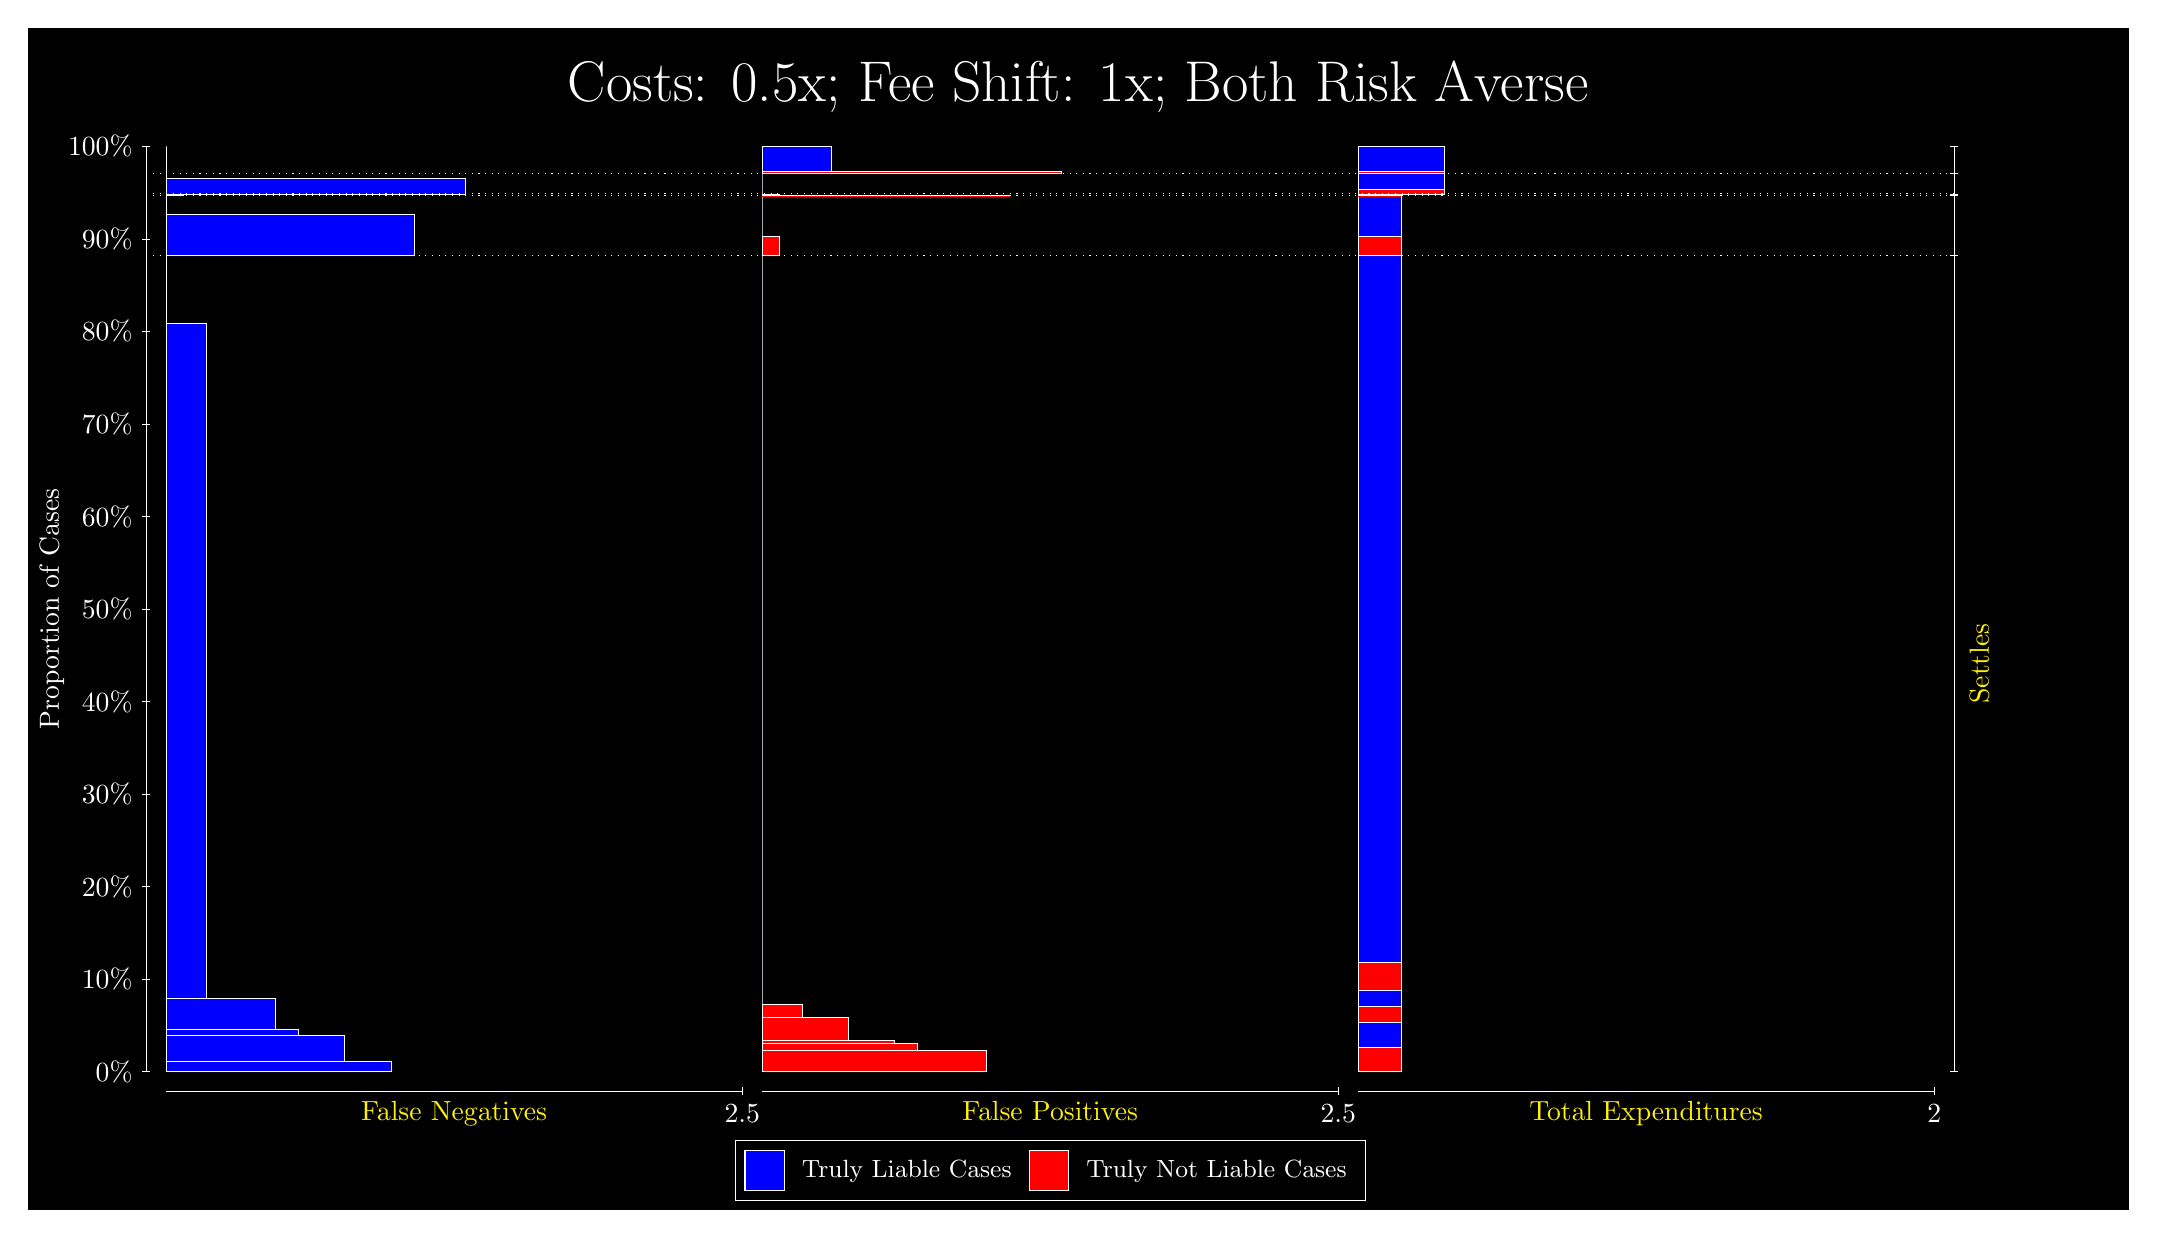
\begin{tikzpicture}
\draw[fill=black] (0,0) rectangle (26.667,15);
\draw[text=white] (0,13.5) rectangle (26.667,15) node[midway] {\huge Costs: 0.5x; Fee Shift: 1x; Both Risk Averse};
\draw[white, very thin] (1.5,1.75) -- (1.5,13.5);
\node[rotate=90, text=white, anchor=center] at (0.3, 7.625) {Proportion of Cases};
\draw[white, very thin] (1.45,1.75) -- (1.55,1.75);
\node[text=white, anchor=east] at (1.45, 1.75) {0\%};
\draw[white, very thin] (1.45,2.925) -- (1.55,2.925);
\node[text=white, anchor=east] at (1.45, 2.925) {10\%};
\draw[white, very thin] (1.45,4.1) -- (1.55,4.1);
\node[text=white, anchor=east] at (1.45, 4.1) {20\%};
\draw[white, very thin] (1.45,5.275) -- (1.55,5.275);
\node[text=white, anchor=east] at (1.45, 5.275) {30\%};
\draw[white, very thin] (1.45,6.45) -- (1.55,6.45);
\node[text=white, anchor=east] at (1.45, 6.45) {40\%};
\draw[white, very thin] (1.45,7.625) -- (1.55,7.625);
\node[text=white, anchor=east] at (1.45, 7.625) {50\%};
\draw[white, very thin] (1.45,8.8) -- (1.55,8.8);
\node[text=white, anchor=east] at (1.45, 8.8) {60\%};
\draw[white, very thin] (1.45,9.975) -- (1.55,9.975);
\node[text=white, anchor=east] at (1.45, 9.975) {70\%};
\draw[white, very thin] (1.45,11.15) -- (1.55,11.15);
\node[text=white, anchor=east] at (1.45, 11.15) {80\%};
\draw[white, very thin] (1.45,12.325) -- (1.55,12.325);
\node[text=white, anchor=east] at (1.45, 12.325) {90\%};
\draw[white, very thin] (1.45,13.5) -- (1.55,13.5);
\node[text=white, anchor=east] at (1.45, 13.5) {100\%};

\draw[white, very thin] (24.457,1.75) -- (24.457,13.5);
\draw[white, very thin] (24.407,1.75) -- (24.507,1.75);
\node[anchor=west] at (24.407, 1.75) {};
\draw[white, very thin] (24.407,12.115) -- (24.507,12.115);
\node[anchor=west] at (24.407, 12.115) {};
\draw[white, very thin] (24.407,12.874) -- (24.507,12.874);
\node[anchor=west] at (24.407, 12.874) {};
\draw[white, very thin] (24.407,12.896) -- (24.507,12.896);
\node[anchor=west] at (24.407, 12.896) {};
\draw[white, very thin] (24.407,13.155) -- (24.507,13.155);
\node[anchor=west] at (24.407, 13.155) {};
\draw[white, very thin] (24.407,13.5) -- (24.507,13.5);
\node[anchor=west] at (24.407, 13.5) {};

\draw[white, very thin, fill=blue] (1.75,1.75) rectangle (4.6044,1.8763);
\draw[white, very thin, fill=blue] (1.75,1.8763) rectangle (4.0188,2.2044);
\draw[white, very thin, fill=blue] (1.75,2.2044) rectangle (3.4333,2.2851);
\draw[white, very thin, fill=blue] (1.75,2.2851) rectangle (3.1406,2.6823);
\draw[white, very thin, fill=blue] (1.75,2.6823) rectangle (2.2623,11.257);
\draw[white, very thin, fill=red] (1.75,11.257) rectangle (1.75,12.115);
\draw[white, very thin, fill=blue] (1.75,12.115) rectangle (4.8971,12.636);
\draw[white, very thin, fill=red] (1.75,12.636) rectangle (1.75,12.874);
\draw[white, very thin, fill=blue] (1.75,12.874) rectangle (1.9696,12.895);
\draw[white, very thin, fill=red] (1.75,12.895) rectangle (1.75,12.896);
\draw[white, very thin, fill=blue] (1.75,12.896) rectangle (5.5558,13.099);
\draw[white, very thin, fill=red] (1.75,13.099) rectangle (1.75,13.155);
\draw[white, very thin, fill=red] (1.75,13.155) rectangle (1.75,13.177);
\draw[white, very thin, fill=blue] (1.75,13.177) rectangle (1.75,13.5);
\draw[white, very thin, fill=red] (9.3189,1.75) rectangle (12.173,2.0239);
\draw[white, very thin, fill=red] (9.3189,2.0239) rectangle (11.295,2.109);
\draw[white, very thin, fill=red] (9.3189,2.109) rectangle (11.002,2.1419);
\draw[white, very thin, fill=red] (9.3189,2.1419) rectangle (10.417,2.4444);
\draw[white, very thin, fill=red] (9.3189,2.4444) rectangle (9.8312,2.6071);
\draw[white, very thin, fill=blue] (9.3189,2.6071) rectangle (9.3189,12.115);
\draw[white, very thin, fill=red] (9.3189,12.115) rectangle (9.5384,12.353);
\draw[white, very thin, fill=blue] (9.3189,12.353) rectangle (9.3189,12.874);
\draw[white, very thin, fill=red] (9.3189,12.874) rectangle (12.466,12.875);
\draw[white, very thin, fill=blue] (9.3189,12.875) rectangle (9.5384,12.896);
\draw[white, very thin, fill=red] (9.3189,12.896) rectangle (9.3189,12.952);
\draw[white, very thin, fill=blue] (9.3189,12.952) rectangle (9.3189,13.155);
\draw[white, very thin, fill=red] (9.3189,13.155) rectangle (13.125,13.177);
\draw[white, very thin, fill=blue] (9.3189,13.177) rectangle (10.197,13.5);
\draw[white, very thin, fill=red] (16.888,1.75) rectangle (17.437,2.0526);
\draw[white, very thin, fill=blue] (16.888,2.0526) rectangle (17.437,2.3807);
\draw[white, very thin, fill=red] (16.888,2.3807) rectangle (17.437,2.5763);
\draw[white, very thin, fill=blue] (16.888,2.5763) rectangle (17.437,2.7833);
\draw[white, very thin, fill=red] (16.888,2.7833) rectangle (17.437,3.1422);
\draw[white, very thin, fill=blue] (16.888,3.1422) rectangle (17.437,12.115);
\draw[white, very thin, fill=red] (16.888,12.115) rectangle (17.437,12.353);
\draw[white, very thin, fill=blue] (16.888,12.353) rectangle (17.437,12.874);
\draw[white, very thin, fill=red] (16.888,12.874) rectangle (17.437,12.875);
\draw[white, very thin, fill=blue] (16.888,12.875) rectangle (17.437,12.896);
\draw[white, very thin, fill=red] (16.888,12.896) rectangle (17.986,12.952);
\draw[white, very thin, fill=blue] (16.888,12.952) rectangle (17.986,13.155);
\draw[white, very thin, fill=red] (16.888,13.155) rectangle (17.986,13.177);
\draw[white, very thin, fill=blue] (16.888,13.177) rectangle (17.986,13.5);
\draw[white, dotted] (1.5,12.115) -- (24.457,12.115);
\draw[white, dotted] (1.5,12.874) -- (24.457,12.874);
\draw[white, dotted] (1.5,12.896) -- (24.457,12.896);
\draw[white, dotted] (1.5,13.155) -- (24.457,13.155);
\draw[white, very thin] (1.75,1.5) -- (9.0689,1.5);
\node[text=yellow, anchor=north] at (5.4094, 1.5) {False Negatives};
\draw[white, very thin] (9.0689,1.45) -- (9.0689,1.55);
\node[text=white, anchor=north] at (9.0689, 1.45) {2.5};

\draw[white, very thin] (9.3189,1.5) -- (16.638,1.5);
\node[text=yellow, anchor=north] at (12.978, 1.5) {False Positives};
\draw[white, very thin] (16.638,1.45) -- (16.638,1.55);
\node[text=white, anchor=north] at (16.638, 1.45) {2.5};

\draw[white, very thin] (16.888,1.5) -- (24.207,1.5);
\node[text=yellow, anchor=north] at (20.547, 1.5) {Total Expenditures};
\draw[white, very thin] (24.207,1.45) -- (24.207,1.55);
\node[text=white, anchor=north] at (24.207, 1.45) {2};

\node[text=yellow, centered, rotate=90] at (24.777, 6.9323) {Settles};





\draw (12.978300999999998,1.5) node[draw=none] (baseCoordinate) {};
\begin{scope}[align=center]
        \matrix[scale=0.5, draw=white, below=0.5cm of baseCoordinate, nodes={draw}, column sep=0.1cm]{
            \node[rectangle, draw, minimum width=0.5cm, minimum height=0.5cm, fill=blue] {}; &
            \node[draw=none, font=\small, text=white] (B) {Truly Liable Cases}; &
            \node[rectangle, draw, minimum width=0.5cm, minimum height=0.5cm, fill=red] {}; &
            \node[draw=none, font=\small, text=white] (B) {Truly Not Liable Cases}; \\
            };
\end{scope}

\end{tikzpicture}
\end{document}